%%%%%%%%%%%%%%%%%%%%%%%%%%%%%%%%%%%%%%%%%%%%%%%%%%%%%%%%%%%%%%%%%%%%%%%%%%%%%%%%
% Limit_Setting.tex: Limit Setting
%%%%%%%%%%%%%%%%%%%%%%%%%%%%%%%%%%%%%%%%%%%%%%%%%%%%%%%%%%%%%%%%%%%%%%%%%%%%%%%%
\chapter{Statistical Analysis and Limit Interpretation}
\label{Limit_Setting_and_Interpretation_Chapter}
%%%%%%%%%%%%%%%%%%%%%%%%%%%%%%%%%%%%%%%%%%%%%%%%%%%%%%%%%%%%%%%%%

%%%%%%%%%%%%%%%%%%%%%%%%%%%%%%%%%%%%%%%%%%%%%%%%%%%%%%%%%%%%%%%%%%%%%%%%%%%%%%%%
\section{Limit Setting}
%%%%%%%%%%%%%%%%%%%%%%%%%%%%%%%%%%%%%%%%%%%%%%%%%%%%%%%%%%%%%%%%%%%%%%%%%%%%%%%%
Since we did not find any excess of events due to a new phenomenon over the expected SM background in our event counting search experiment, we need to make important quantitative statements which are based on the negative finding and will be useful to other particle physicists or future experiments. The expected new phenomenon described by the SPS8 benchmark GMSB model is the decay of the lightest neutralino~(\PSneutralinoOne) into a late photon and a gravitino which can be observed in events with a late photon and large missing transverse energy. An exclusion limit~(is either an "upper" or "lower" limit) is an important quantitative statement on the lifetime, mass of the \PSneutralinoOne and the product of its production cross section and branching ratio. It allows us to make statements like the following: 
\begin{itemize}
\item a lightest neutralino, if it exists, is produced with a cross section below a certain threshold, with this probability, and the certain threshold is an \textbf{upper} limit on the lightest neutralino production cross section.
\item a lightest neutralino decay, if it happens, takes place with a mean lifetime larger than a certain threshold, with this probability, and this threshold is a \textbf{lower} limit on the neutralino mean lifetime.
\end{itemize}
%%%%%%%%%%%%%%%%%%%%%%%%%%%%%%%%%%%%%%%%%%%%%%%%%%%
We evaluate an exclusion limit for the lightest neutralino decay to photon and gravitino using a method for deriving an exclusion limit from the \textit{Confidence Interval} or \textit{Confidence Limit}~(CL) known as the \textit{modified frequentist approach} or the $CL_{s}$ method.  This method uses the number of observed events, the expected background events, the expected signal events according to the SPS8 benchmark GMSB model and the systematic uncertainties to compute 95\% CL on the cross section which can be translated into exclusion limits on the mean lifetime, $\tau_{\PSneutralinoOne}$~(ns), and the mass of the  \PSneutralinoOne, $m_{\PSneutralinoOne}$~(\GeVcc),  or the effective SUSY breaking scale, $\mathbf{\Lambda}$~(\TeV). %We also produce a two dimensional limit in $\tau_{\PSneutralinoOne}$ and $m_{\PSneutralinoOne}$~(\GeVcc) still using the CLs technique.
%%%%%%%%%%%%%%%%%%%%%%%%%%%%%%%%%%%%%%%%%%%%%%%%%%%%%%%%%%%%%%%%%%%%%
%%%%%%%%%%%%%%%%%%%%%%%%%%%%%%%%%%%%%%%%%%%%%%%%%%%%%%%%%%%%%%%%%
\subsection{Signal Efficiency and Acceptance}
%%%%%%%%%%%%%%%%%%%%%%%%%%%%%%%%%%%%%%%%%%%%%%%%%%%%%%%%%%%%%%%%%
The plot in Figure \ref{fig:EffAcc} show our signal selection efficiency and acceptance for signal events of MC samples with different mean lifetime in \mm or \textit{proper decay length}, $c\tau$, ranging from 500\mm to 6000\mm with the same lightest neutralino mass of 255\GeVcc or effective SUSY breaking scale $\mathbf{\Lambda=180}$\TeV. 

\vspace{5mm}
\begin{minipage}{0.90\linewidth} 
\begin{center}
%\mbox{
%\includegraphics[width=0.49\textwidth,height=0.5\textwidth]
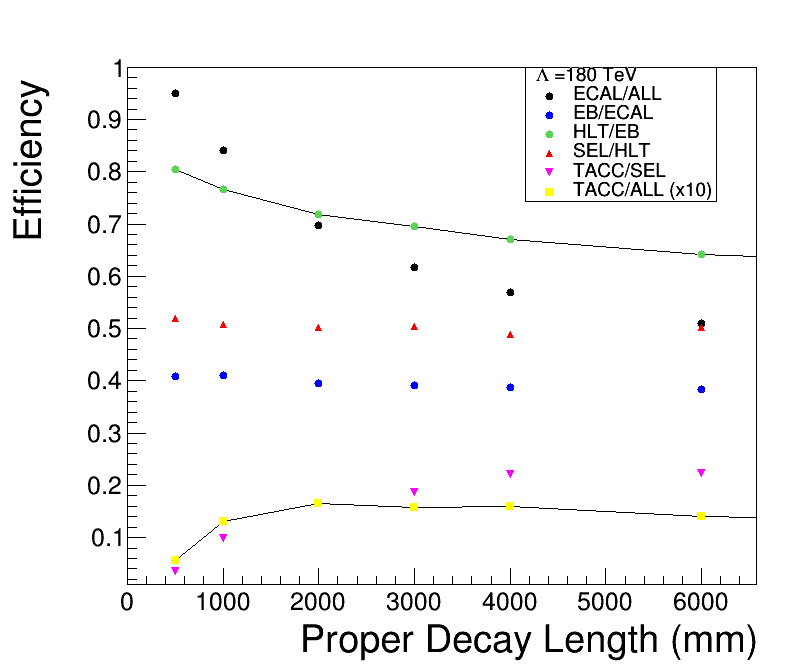
\includegraphics[height=0.65\textwidth, width=0.8\textwidth]{THESISPLOTS/Eff_180_ctau_2015.png}
%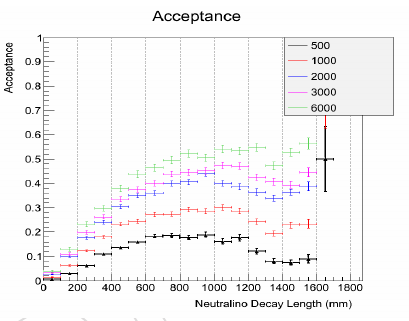
\includegraphics[height=0.5\textwidth, width=0.5\textwidth]{THESISPLOTS/SignalReconstructionAcceptance.png}}
\captionof{figure}{The efficiency for different mean decay length, $c\tau$~[\mm] with  $\mathbf{\Lambda=180}$\TeV. TACC/ALL~(yellow square markers) is the  Efficiency $\times$ Acceptance($t>3$~ns) \ie $\varepsilon \times A$, used in evaluating the exclusion limits. }
\label{fig:EffAcc}
\end{center}
\end{minipage}

\vspace{5mm}
The efficiency times acceptance~($\varepsilon \times A$) used in Equation \ref{eq:SIGMAUPA} to evaluate the exclusion limits is the TACC/ALL which is the ratio of the events passing our event selection with photon time, $t > 3$~ns in the barrel to all events with photons from the decay of the generated lightest neutralino. The $\times 10$  factor for TACC/ALL shown on the plot  is only for display purpose and was not used in evaluating the limits. 
\newline
The efficiency times acceptance, is small~(less than 10\%) for smaller values of $c\tau = 500\mm$~($\tau = 1.7$~ns) since very few of the events with photon from the lightest neutralino decay have time, $t > 3$~ns, despite many of photons reaching ECAL as is seen in the ECAL/ALL~(ratio of events with photons reaching ECAL to all events with photons from the decay of the generated lightest neutralino.) where the efficiency times acceptance is high for low $c\tau$ values. 
\newline
The efficiency times acceptance shown in Figure \ref{fig:EffAcc} peaks at $c\tau = 2000\mm$~($\tau = 6.7$~ns) and then begins to slightly fall for larger $c\tau$ values. For very large $c\tau > 6000\mm$ values not shown on the plots, the efficiency times acceptance is again less than 10\% since most of the lightest neutralinos decay outside of the ECAL and are undetected, as seen in the ECAL/ALL where the efficiency keeps dropping with increased $c\tau$ values.

\subsection{Systematic Studies}
We have required in our event selection that the photon \pt is greater than 80\GeVc, the jet \pt is greater than 35\GeVc and the missing energy is greater than 60\GeV. The same selection requirements applied to our MC signal event sample should guarantee a good event selection efficiency estimate. Any difference in the photon \pt, jet \pt and missing transverse energy between MC and data, will be a source of systematic uncertainties on the efficiency of selecting signal events. These uncertainties can come from quantities like jet energy scale~(JES), jet energy resolution~(JER), electron-photon energy scale, instrumentation related and energy deposits not clustered during missing transverse energy reconstruction, photon ECAL arrival time bias and ECAL time resolution. 
\newline
Table \ref{tab:SYST} presents the sources of uncertainties considered in this analysis. These uncertainties are computed by varying the nominal values of each quantity, while keeping the others fixed, by $1\sigma$ deviation and counting the number of events passing our event selection requirements. ECAL timing bias which has to do with the absolute reference time~(zero ns) of the ECAL timing, is the source of our largest uncertainty. The photon arrival time is measured with respect to this reference time. This ECAL time uncertainty has the largest impact on our analysis, since our analysis is based on counting the number of events with photon ECAL time above $3$~ns. The next largest uncertainties are from energy deposits missed by the clustering algorithm. This affects the photon energy scale, missing energy scale,  jet energy scale and resolution.
The uncertainty on the photon energy scale in the barrel was estimated to be 4.0\%  which is based on measuring the photon energy of events with $Z\rightarrow \mu\mu\gamma$ decay, where the muon radiates a photon in a process known as the final-state radiation~(FSR) \cite{PES}.  
\newline
The uncertainty on the \MET resolution uses a conservative estimate from \MET measurements in QCD events \cite{METRES}, where the \MET uncertainty is calculated using the fraction of events passing an event selection based on \MET for varying thresholds of \MET. 
\newline
The uncertainty on the ECAL time resolution was obtained by comparing the mean time of photons of events from $\gamma +$ jet MC sample to events from data with photon ECAL time, $|t_{\gamma}| < 2$~ns. The difference is found to be of the order of 200~ps per event. 
\newline
Meanwhile, the systematic uncertainty on luminosity measurement has the recommended value of $2.2$\% provided by CMS and LHC luminosity measurements while the uncertainty from Parton Density Functions~(PDF) is evaluated using the re-weighting technique which uses the Master Equation of CTEQ65 model set described in \cite{PDF}.
\newline
Since our background estimation is data-driven, the systematic uncertainties do not impact our results in a significant way.
The statistical uncertainty in the \textsf{ABCD} background estimation method is our largest source of uncertainty in this analysis and we estimate it to vary upward by 223\% and downward by 51\%. This large background statistical uncertainty is because of the very low event yields. Our final result is affected by the signal selection efficiency only, despite the large background estimation uncertainty. These signal selection uncertainties are used as nuissance parameters in the calculation of the upper limit on the observed signal cross section~($\sigma_{UL}$).

\vspace{5mm}
\begin{minipage}{0.90\linewidth} 
\begin{center}
%\begin{table}[ht]
%\renewcommand\arraystretch{1.2}
\begin{tabular}{c c}
\toprule
\hline
\bfseries{Source} & \bfseries {Uncertainty(\%)}\\
\hline
\toprule
\texttt{ECAL absolute time }~(0.0~ns) & $<10.0$\% \\
\texttt{ECAL time resolution}~(0.5~ns) & $<5.0$\% \\
\texttt{Unclustered energy deposits} & $<9.0$\% \\
\texttt{Photon energy scale}  & $< 4.0$\% \\
\texttt{Jet energy scale}~(JES)  & $< 9.0$\% \\
\texttt{Jet energy resolution}~(JER) &$ <9.0$\% \\
\texttt{\MET resolution} & $ <2.8$\%  \\
\texttt{PDF uncertainty} & $< 1.70$\% \\
\hline
\toprule
\texttt{Background estimation uncertainty} &$51.0$\% to 223\% \\
\hline 
\texttt{Luminosity}~(4.5\%) & $< 2.2$\% \\
\hline
\bottomrule
\end{tabular}
\captionof{table}{Summary of systematic uncertainties for signal efficiency and background estimation in this analysis and applied to our final results.}
\label{tab:SYST}
%\end{table}
\end{center}
\end{minipage}

%%%%%%%%%%%%%%%%%%%%%%%%%%%%%%%%%%%%%%%%%%%%%%%%%%%%%%%%%%%%%%%%%%%%%%%%%%%%%%%%%%%%%%%%%%%%%%%%%%%%%%%%
\subsection{Statistical Test Formalism}
In order to compute the exclusion limits, we perform a statistical inference on the Alternate hypothesis, $H_{1}$, which is the SPS8 benchmark GMSB model. Since the result of our search was negative, we try to exclude a region in a parameter space of the SPS8  benchmark GMSB model which do not pass the goodness-of-fit test to the observed data. A set of values of the \textit{Parameter Of Interest}~(POI) describing the SPS8 benchmark GMSB model is excluded if the corresponding evaluated value of the $CL_{s}$ is below $0.05$, which corresponds to 95\% of confidence level~(CL).
\par 
Since our search experiment is an event counting experiment, we construct a histogram, in the photon ECAL time, of the number of events, $\mathbf{M}$, passing our final event selection and acceptance. Suppose the number of events in each bin of the histogram is $n_{i}$,  with $i = 1, \cdots, N$, where $N$ is the number of bins of the histogram. The expected number of events in the $i^{th}$ bin, $E[n_{i}]$, is the sum of events from all known physics processes which is a combination of events due to the Standard Model, which we  call background events, $b_{i}$, and events due to the  SPS8 benchmark GMSB model, which we call signal events, $s_{i}$. Thus, the expected number of events in the $i^{th}$ bin is given as
\begin{equation}
 E[n_{i}] = \mu s_{i} + b_{i}
\end{equation}
where $\mu$ is the  POI which is the \textit{signal strength}. It relates the expected cross section~($\sigma_{th}$) according to the SPS8  benchmark GMSB model and the actual observed cross section~($\sigma^{Obs}$) through 
\begin{equation}
\mu = \frac{\sigma^{Obs}}{\sigma_{th}}.
\end{equation}
When $\mu = 0$, it means the  SPS8  benchmark GMSB model had no contribution to the number of events in each bin and provides a test for the Standard Model background-only hypothesis. When $\mu=1$, it means the SPS8  benchmark GMSB theory contributed to the number of events as expected and this provides a tests for the signal plus background hypothesis. The other values for $\mu$ corresponds to different rates of the SPS8 benchmark GMSB model.
\par 
The exclusion limits of $\mu$ can be derived from the \textit{test statistics}, which is a function of $\mu$, of the alternate hypothesis under testing. There are many different ways to construct a test statistics, however, the CMS statistics committee recommends the \textbf{profile likelihood ratio} as the test statistics to be used in a search and discovery experiment and according to the Neyman-Pearson theorem, the profile likelihood ratio gives the most powerful hypothesis test \cite{NPT}. 
The profile likelihood ratio is computed from the likelihood function for the histogram. This likelihood function, $\mathcal{L}$, is the product of the Poisson probabilities for all the bins of the histogram:
\begin{equation}\label{eq:LL}
\mathcal{L}\left( \mu, \mathbf{\theta} \right) = \prod^{N}_{i=1} \frac{{\left( \mu s_{i} + b_{i} \right)}^{n_{i}}}{n_{i}!} e^{-(\mu s_{i} + b_{i})} \cdot \mathcal{G}(\mathbf{\theta} ),
\end{equation}
where $\mathcal{G}(\mathbf{\theta})$, is a discrete~(Poisson) distribution of the \textit{nuisance parameters} through which the systematic uncertainties due to efficiency of the signal events and the integrated luminosity and the theory uncertainties which can impact the final result on $\mu$ can be introduced. If the profile likelihood is plotted as a function of $\mu$, the nuisance parameter will cause broadening of the distribution of the profile likelihood and this reflects the loss in sensitivity or loss of information about the parameter $\mu$, due to the systematic uncertainties.
%The distribution can be different for different nuisance parameter since $\mu$ is also dependent of $\theta$.
\newline
Using the likelihood function, the profile likelihood ratio~(for simplicity, instead of writing the explicit dependence of $\mathcal{L}$ on $n_{i}$, we write  $\mathcal{L}$ in terms of the parameters) is defined as
\begin{equation}\label{eq:PLL}
\lambda(\mu) =  \frac{\mathcal{L}(\mu, \hat{\hat{\mathbf{\theta}}})}{\mathcal{L}(\hat{\mu}, \hat{\mathbf{\theta}} )}
\end{equation}
where $\hat{\hat{\mathbf{\theta}}}$, known as the \textit{conditional maximum-likelihood estimator}~(CMLE) of $\mathbf{\theta}$, is the the value of $\mathbf{\theta}$ that maximizes $\mathcal{L}$ for a fixed value of $\mu$, and it is a function of $\mu$.  $\mathcal{L}(\hat{\mu}, \hat{\mathbf{\theta}} )$ is the maximized (unconditional) likelihood function with $\hat{\mu}$ and $\hat{\mathbf{\theta}}$ being its \textit{maximum likelihood}~(ML) estimators. 
\newline
We are interested in estimating an interval for the parameter $\mu$.
\newline
In our statistical inference test, we use only a single bin, which means $N = 1$, in the expected signal, estimated background and data histograms since we observed only one event passing our final event selection.
\subsubsection{Test statistics and $p$-values} 
The expression for $\lambda(\mu)$ given in Equation \ref{eq:LL}, suggest that $0 \leq \lambda \leq 1$. When $\lambda$ is close to 1, it means a very good agreement between the data and the given hypothesis defined by the value of $\mu$.  Using $\lambda(\mu)$, the test statistics is defined as
\begin{equation}
 q_{\mu} = -2\ln \lambda(\mu) .
\end{equation}
\par 
The test statistics approach to hypothesis testing is very favorable because of its very simple interpretation: higher values of the test statistics corresponds to increasing incompatibility between the data and signal plus background hypothesis and this incompatibility can be quantified by calculating a $p$-value, which is \textit{probability of compatibility} from the test statistics. 
\newline
Using the observed data, this probability or confidence interval is evaluated as 
\begin{equation}
 CL^{(\mu)}_{s+b} = p_{s+b} = \int^{\infty}_{q^{obs}_{\mu}} f(q_{\mu}|\mu) dq_{\mu},
\end{equation}
where, $q^{obs}_{\mu}$, is the value of the test statistics~($q_{\mu}$) from data.
$f(q_{\mu}|\mu)$ is a probability density function~(pdf) of the test statistic. The notation for the pdf, $f(q_{\mu}|\mu^{\prime})$, is interpreted as the pdf for the test statistics, $q_{\mu}$, computed for a sample of events generated through Monte Carlo event generation with the assumption that $\mu = \mu^{\prime}$. 
\newline
For the background-only scenario, the test statistics with $\mu = 0$, is re-written as
%\begin{equation}\label{eq:HNULL}
\[\label{eq:HNULL}
 q_{\mu} = \left\lbrace  
  \begin{array}{ll}
 -2\ln \lambda(0), & \hat{\mu} \geq 0 \\
   0,              & \hat{\mu} \leq 0
  \end{array}
  \right.
\]
where, $\lambda(0)$, is the profile likelihood ratio for $\mu = 0$, defined in Equation \ref{eq:PLL}.
The probability for the background-only~($\mu = 0$) hypothesis being compatible with the data, $ CL^{(\mu)}_{b}$  is defined as
\begin{equation}\label{eq:HALT}
 CL^{(\mu)}_{b} = 1 - p_{b} = \int^{\infty}_{q^{obs}_{\mu}} f(q_{\mu}|0) dq_{\mu},
\end{equation}
where, $f(q_{\mu}|0)$, denotes the pdf of the test statistics, $q_{\mu}$, under the background-only~($\mu = 0$) hypothesis.
Using Equation \ref{eq:HNULL} and \ref{eq:HALT}, the \textbf{observed} confidence limit or probability, $ CL^{(\mu)}_{s} $ is evaluated as
\begin{equation}
CL^{(\mu)}_{s} = \frac{CL^{(\mu)}_{s+b} }{ CL^{(\mu)}_{b}}.
\end{equation}
By increasing the value of $\mu$~(increasing the contribution of the signal), the $CL^{(\mu)}_{s}$ decreases, and the value $\mu^{UL}$ for which $CL^{(\mu^{UL})}_{s} = \alpha$ is the observed \textbf{upper limit} for $\mu$ at the required confidence level $1 - \alpha$. In the case of our 95\% confidence interval, $\alpha = 0.05$
\newline
In practice, the pdfs $f(q_{\mu}|\mu)$ and $f(q_{\mu}|0)$ of the test statistics for signal plus background and  background-only hypothesis, respectively, are obtain for the different values of $\mu$, until the value of $\mu$ which gives the upper limit is obtained. The pdfs are evaluated through Monte Carlo samples generated for the cases with arbitrary $\mu $ and $\mu = 0$, respectively, and their $p$-values are the area under each pdf bounded from below by the observed value of the test statistics from data, $q^{obs}$.
\newline
The \textbf{expected} exclusion limit of the SPS8 benchmark GMSB hypothesis is obtained using the median of the test statistics from producing toy search experiment through Monte Carlo simulation and gives the initial sensitivity of the experiment.  
\subsection{HiggsCombine Tool}
In CMS, the $CL_{s}$ method for hypothesis testing and evaluating confidence limits has been implemented in a statistical software package called \textit{HiggsCombine} \cite{LIMITS}. The Higgscombine tool provides access to a variety of robust statistical methods with optimized performance for computing limits. The HiggsCombine tool takes as input the expected number of events or histogram of signal and estimated  background, the observed number of events or histogram from data, estimates or histogram of the uncertainties and produce an upper limit in the production cross section of a given physics process for a given value of a parameter of interest~(POI). In addition to the numerous computing and optimization advantages, the Higgscombine tool allows for the possibility of using several different statistical inference methods like Frequentist, Bayesian, Analytical and Hybrid methods to calculate the upper limit. This way, one can make comparison and simple checks for any inconsistency. In this analysis, we used an Asymptotic method for testing and the HybridNew~(a hybrid of Frequentist and Bayesian methods) method  to evaluate our final observed  limits \cite{LIMITS,ASYMP}. 

%%%%%%%%%%%%%%%%%%%%%%%%%%%%%%%%%%%%%%%%%%%%%%%%%%%%%%%%%%%%%%%%%%%%%%%%%%%%%%%%%%%%%%%%%%%%%%%%%%%%%%%%%%%%%%%%%
%%#######################################################################################################
\section{Limit Interpretation in the SPS8 Benchmark GMSB Model}
\textbf{Explain here what the observed, expected and standard deviation limits are and what they are used for}
\newline
\textbf{Also explain the excluded regions excluded this far.}
\par 
In addition to the \textbf{observed} limit~(shown as a solid black line in Figure \ref{fig:SPS8_Ctau_Ulimit}), we also evaluate the uncertainties on the \textbf{expected} or median~(50\%) limit~(dashed red line) at 68\%~($+ 1\sigma$) or 16\%~($- 1\sigma$) and at 98\%~($+ 2\sigma$) or 2.5\%~($- 2\sigma$) shown with the \textcolor{green}{GREEN} and \textcolor{yellow}{YELLOW}  bands, respectively, in the same Figure \ref{fig:SPS8_Ctau_Ulimit}.
\newline
Using  the upper limits in $\tau$ and mass of the lightest neutralino or effective SUSY breaking scale, $\mathbf{\Lambda}$, we produce a two dimensional exclusion limit in $\tau$ and $\mathbf{\Lambda}$ and also a cross section limit according to the SPS8 benchmark GMSB model. 
%%%%%%%%%%%%%%%%%%%%%%%%%%%%%%%%%%%%%%%%%%%%%%%%%%%%%%%%%%%%%%%%%%%%%%%%%%%%%%%%%%%%%%%%%%%%%%%%%%%%%%
\subsection{Cross Section and Branching Ratio Limits}
From the \texttt{HiggsCombine}, we obtain an upper limit on parameter of interest, $\mu^{UL}$ or observed number of events, $N^{Obs}$). Using the efficiency and acceptance the upper limit on the observed number of events can be the observed upper limit on the cross section given as 
\begin{equation}{\label{eq:SIGMAUPA}}
\sigma^{Obs}_{UL} = \frac{\mu^{UL} \cdot N^{Expt}}{\varepsilon\times A\cdot \mathscr{L}}
\end{equation}
where, $\mathscr{L}$, is the integrated luminosity~(19\fbinv) and $\varepsilon$ and $A$ are the signal selection Efficiency and Acceptance, respectively and we have used the relationship between the cross section~($\sigma$) the number of events~($N$): $\sigma = \frac{N}{\varepsilon\times A \cdot \mathscr{L}}$.
\newline
If the effective SUSY breaking scale is $\mathbf{\Lambda} = 180\TeV$ then the upper limit on the product of the lightest neutralino production cross section and branching ratio decay to a photon and gravitino channel, $\PSneutralinoOne \rightarrow \gamma + \tilde{G}$, according to the SPS8 benchmark GMSB model is, $\sigma\times BR = 12.05$~fb. The mean lifetime of the lightest neutralino $\tau_{\PSneutralinoOne}$, is either less than $3.2$~ns or larger than 19.87~ns as shown in right plot of Figure \ref{fig:SPS8_Ctau_Ulimit}.
\newline
For a given lightest neutralino mass and mean lifetime, we can also find its corresponding excluded cross section using Figure \ref{fig:SPS8_SIGMA-Ulimit}. For example, lightest neutralinos with mass,  $m_{\PSneutralinoOne} = 255\GeVcc$, or effective SUSY breaking scale,  $\mathbf{\Lambda} = 180\TeV$, and mean lifetime, $\tau_{\PSneutralinoOne} = 10.0$~ns, have an observed upper limit on their production cross section times branching ratio in the decay to photon and gravitino channel of $\sigma^{UP}_{\PSneutralinoOne} \geq 0.01$~pb at 95\% CL.
%%%%%%%%%%%%%%%%%%%%%%%%%%%%%%%%%%%%%%%%%%%%%%%%%%%%%%%%%%%%%%%%%%%%%%%%%%%%%%%%%%%%%%%%%%%%%%%%%%%%%%%%
\subsection{Mass and Lifetime Limits}
Using the cross section from theory~(shown as the blue line in Figure \ref{fig:SPS8_Ctau_Ulimit}, for example), the excluded region in the mean lifetime of the lightest neutralino according to the SPS8 benchmark GMSB model are the values of mean lifetime, $\tau$, for which the observed cross section is below the theory cross section, \ie a lower limit and an upper limit on $\tau$ is extracted for the corresponding points where the observed cross section and the theory cross section intersect.
An exclusion  upper limit on the mass or effective SUSY breaking scale, $\mathbf{\Lambda}$, is obtained from Figure \ref{fig:MASS-limits} at the point where the observed cross section~(solid black line) intersects with the expected~(blue line) cross section. 
\newline
The excluded lightest neutralino mass, $m_{\PSneutralinoOne}$, or effective SUSY breaking scale, $\mathbf{\Lambda}$, observed from the cross section against lightest neutralino mass plot of Figure \ref{fig:MASS-limits} for $\tau = 6.7$~ns is up to  $m_{\PSneutralinoOne} = 300\GeVcc$ or  $\mathbf{\Lambda} = 220\TeV$, still in the context of the SPS8 benchmark GMSB model.
\newline
From the 2 dimensional plane define by $(\mathbf{\Lambda},\tau_{\PSneutralinoOne})$ of the exclusion limit, shown in  Figure \ref{fig:SPS8_2D-Ulimit}, the excluded lightest neutralino mean lifetime, $\tau_{\PSneutralinoOne}$, is from $2.0$~ns to $45.0$~ns for low mass~($m_{\PSneutralinoOne} < 150\GeVcc$) lightest neutralino. This exclusion in mean lifetime shrinks as the mass of the lightest neutralino increases or effective SUSY breaking scale increases. This is because the production cross section for the lightest neutralino decreases with increase in its mass or $\mathbf{\Lambda}$. 

\vspace{5mm}
\begin{minipage}{0.90\linewidth}
\begin{center}
%\mbox{
%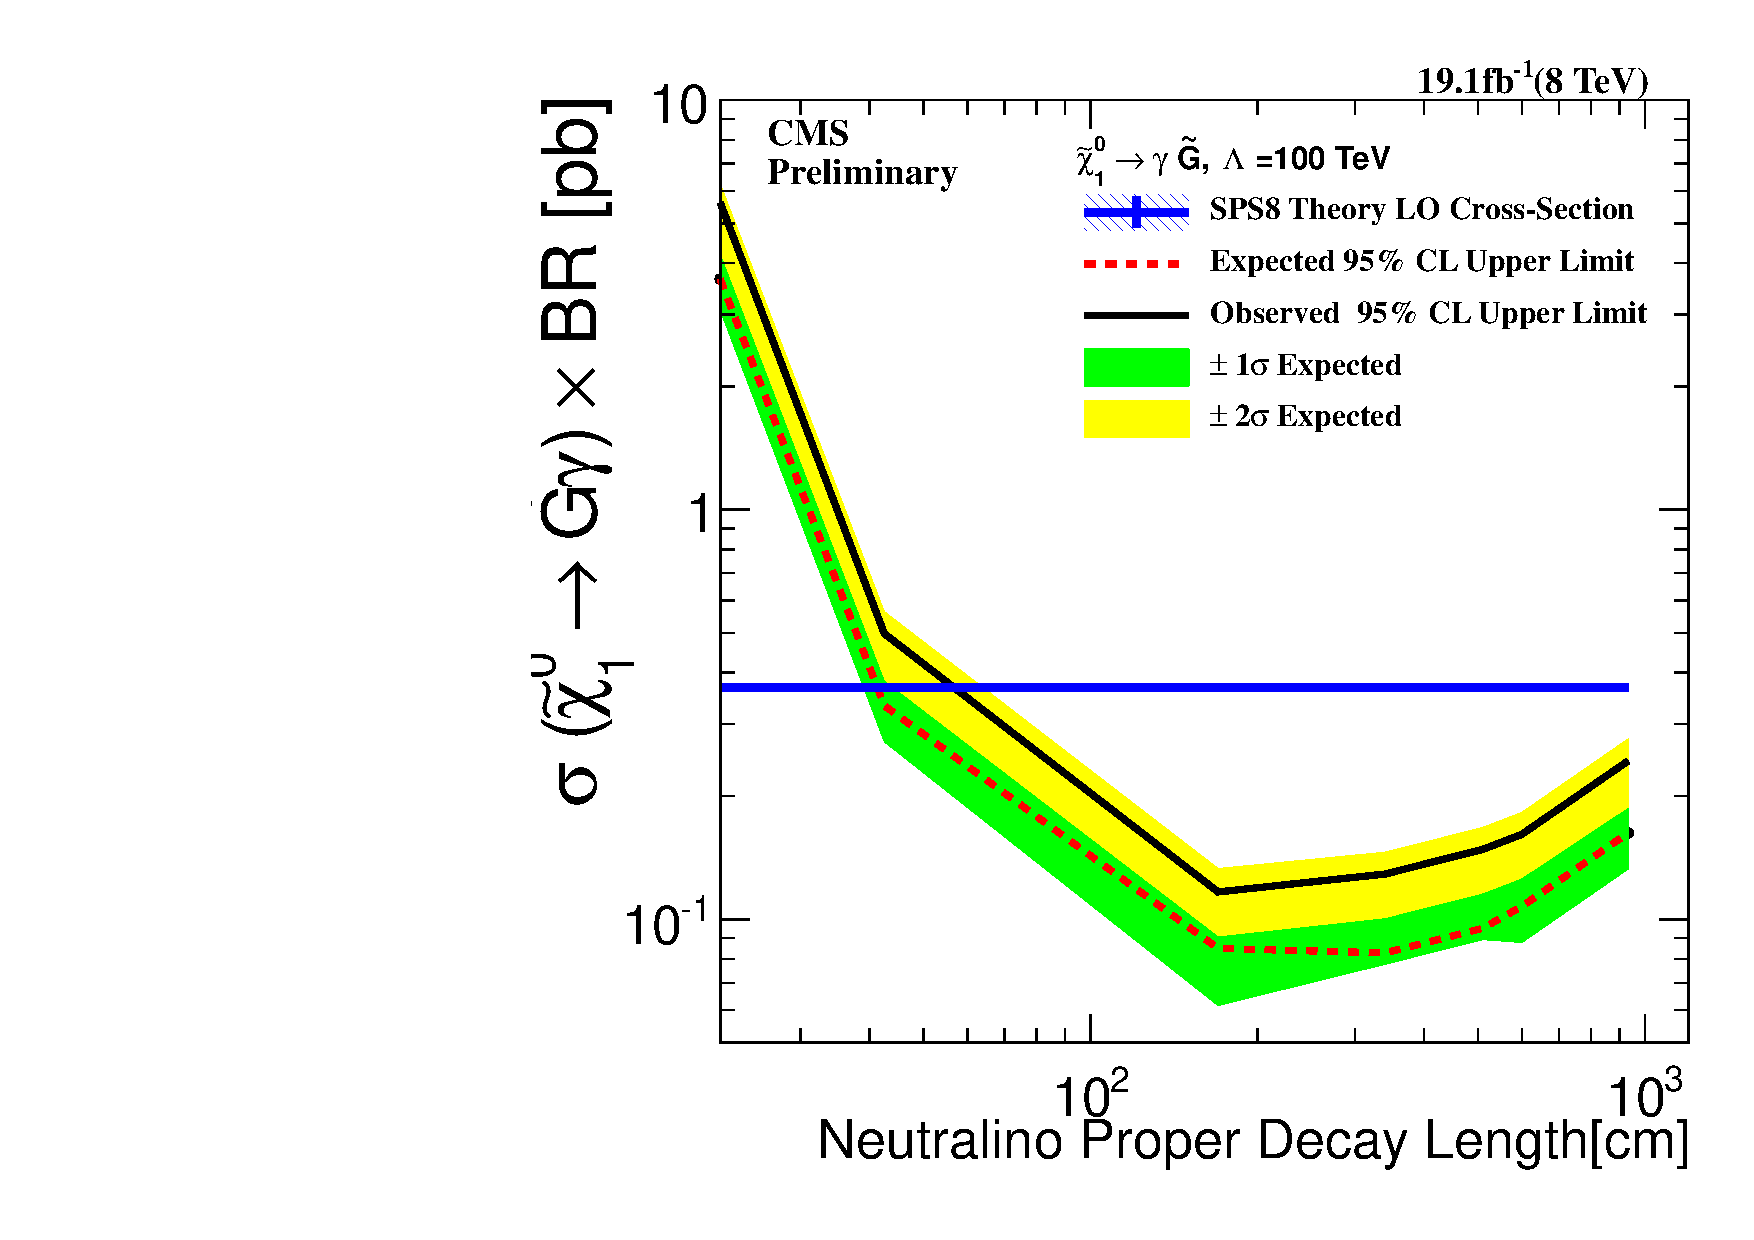
\includegraphics[height=0.65\textwidth, width=0.53\textwidth]{THESISPLOTS/100TeV_Neutralino_CrossSecTimesBR_Uplimit.pdf}
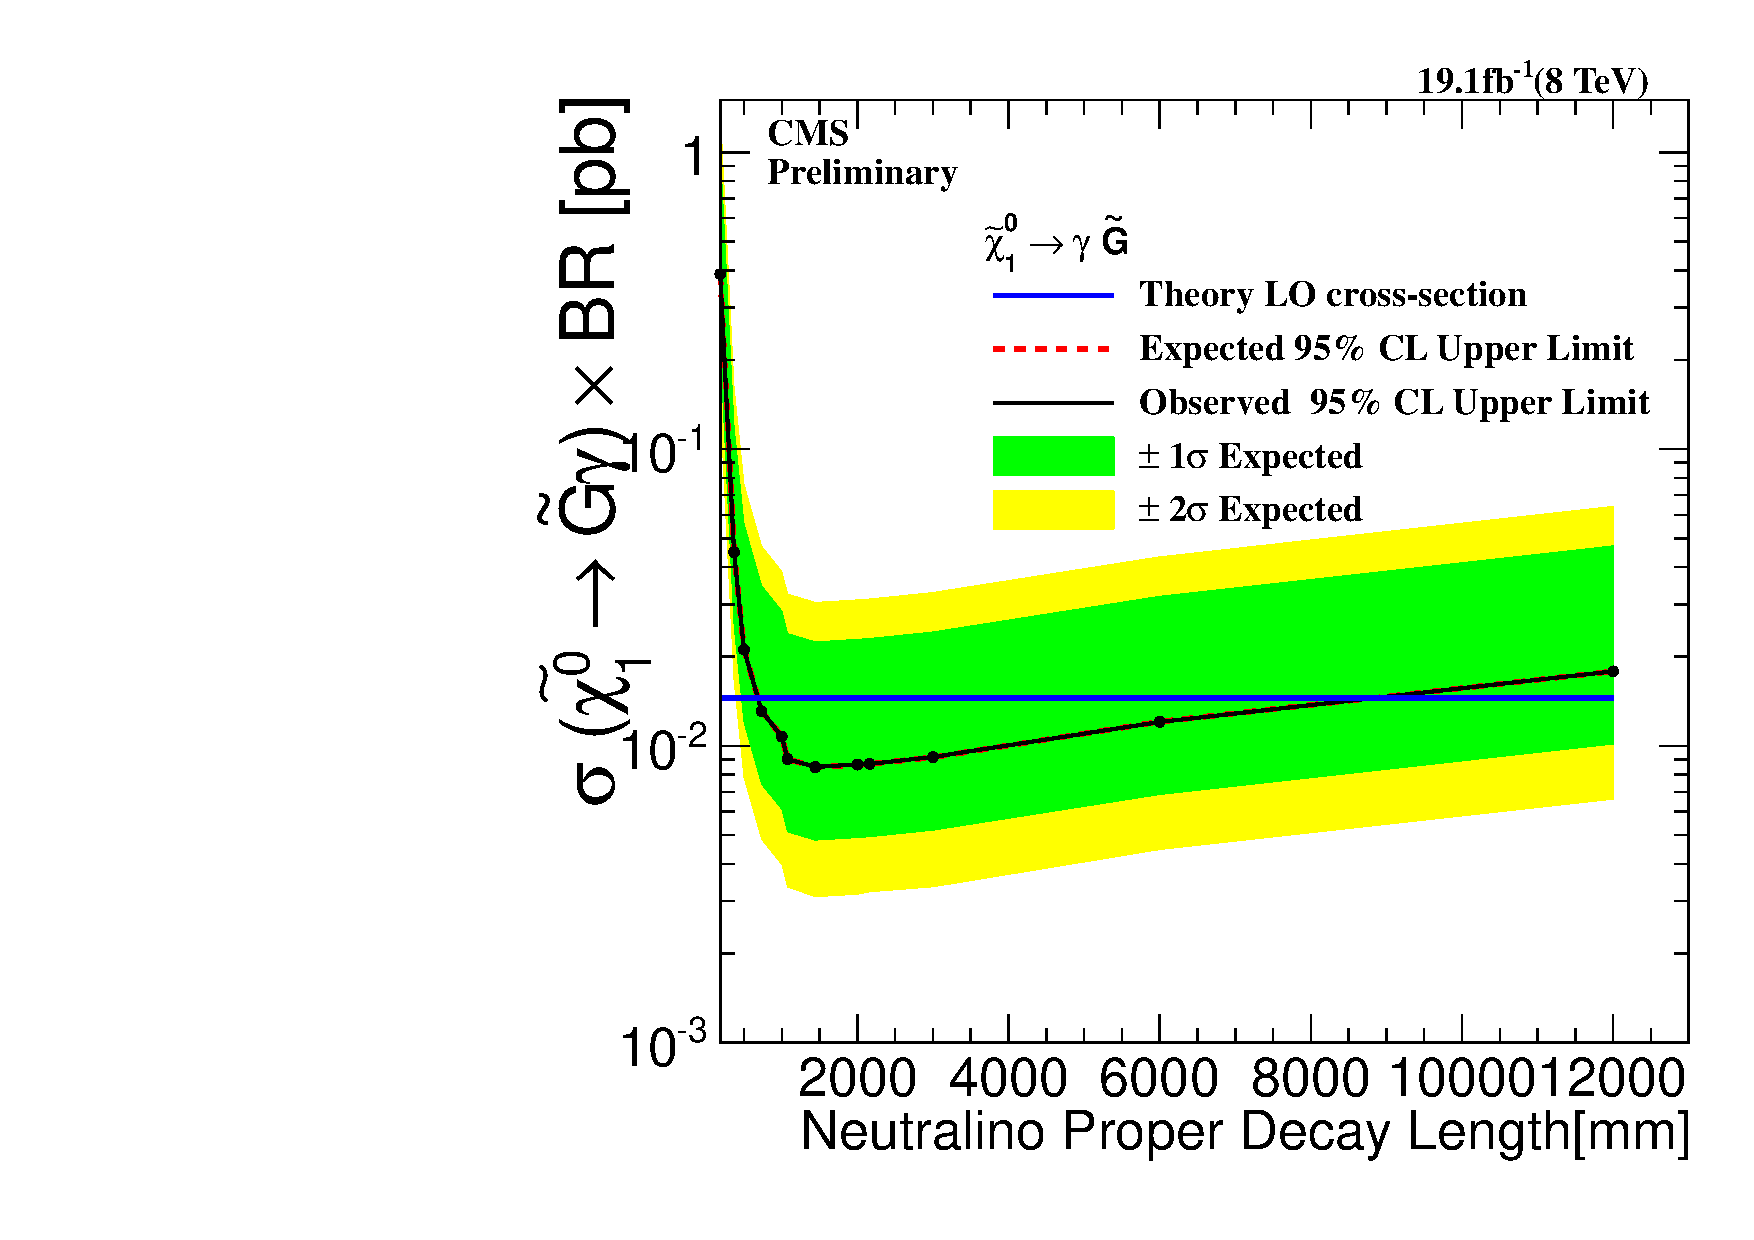
\includegraphics[height=0.8\textwidth, width=0.85\textwidth]{THESISPLOTS/Neutralino_CrossSecTimesBR_Uplimit.pdf} 
%}
\captionof{figure}{ 95\% CL evaluated using the $CL_{s}$ procedure on the lightest neutralino production cross section times branching ratio~($\sigma\times BR$) against mean lifetime~(ns) for $\mathbf{\Lambda = 180}$\TeV in the SPS8 benchmark GMSB model.}
\label{fig:SPS8_Ctau_Ulimit}
\end{center}
\end{minipage}
\vspace{5mm}

\vspace{5mm}
%\begin{figure}[!htb]
\begin{minipage}{0.90\linewidth}
%%\afterpage{ %
 %% \clearpage% Flush earlier floats (otherwise order might not be correct)
   %% \thispagestyle{empty}% empty page style (?)
%%\begin{landscape}% Landscape page
\begin{center}
%\mbox{
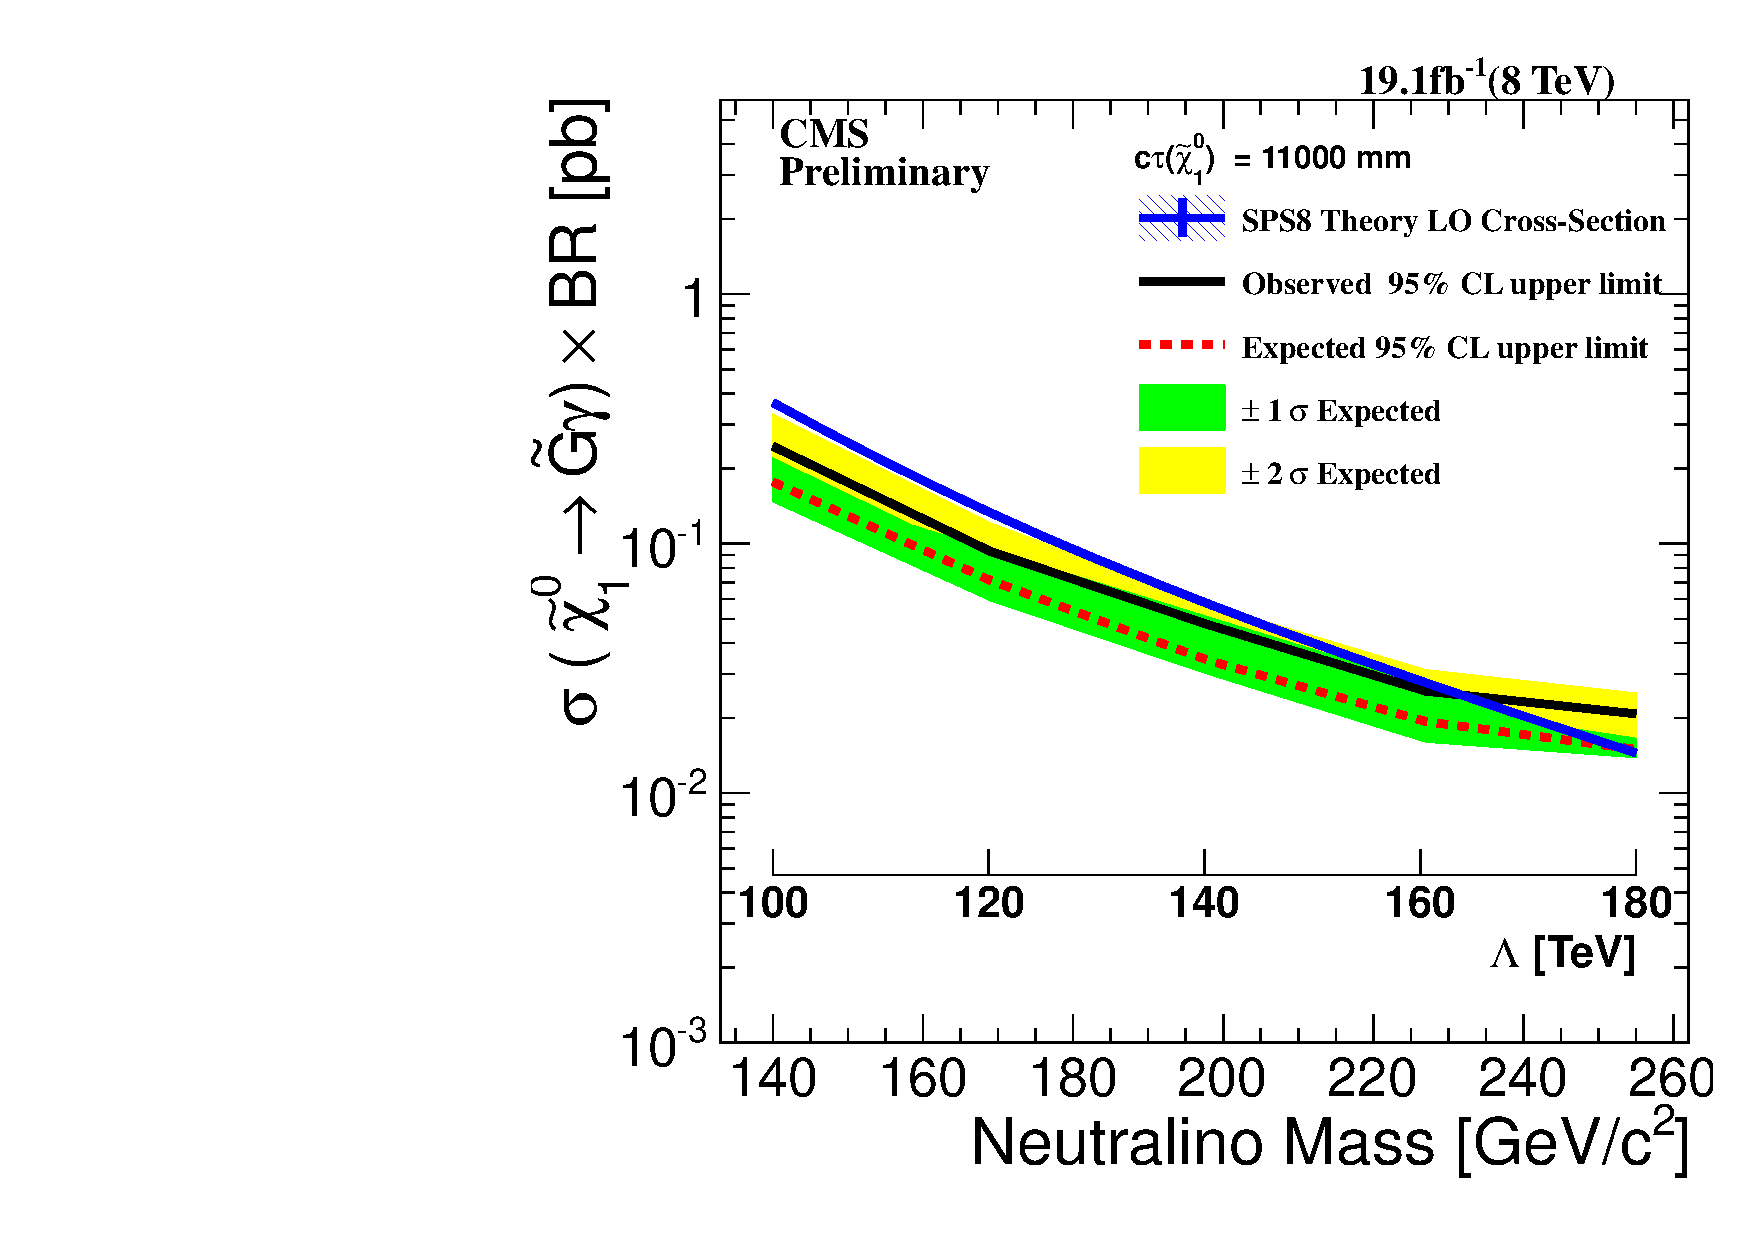
\includegraphics[height=0.8\textwidth, width=0.85\textwidth]{THESISPLOTS/Neutralino_CrosSecVsMass_Exclusion_limit_11000.pdf}
%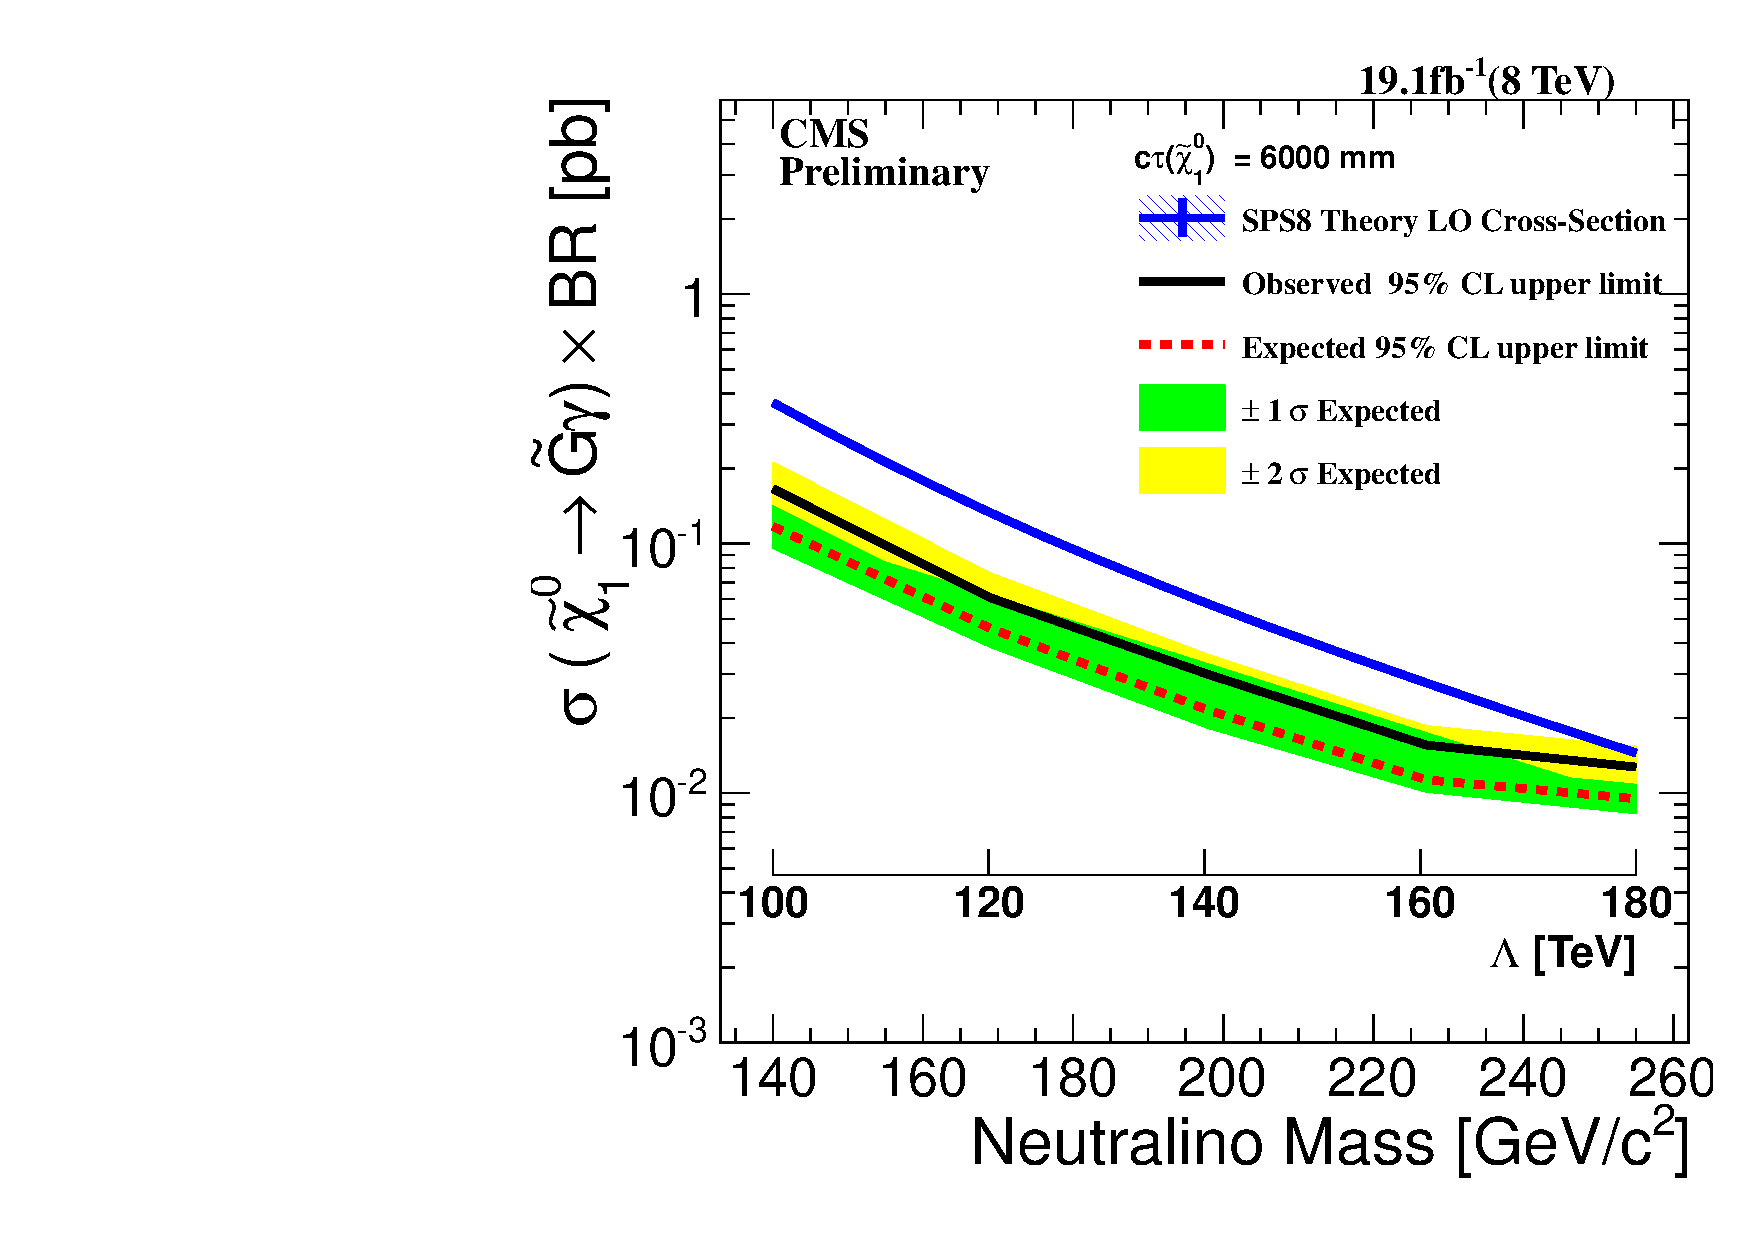
\includegraphics[height=0.65\textwidth, width=0.53\textwidth]{THESISPLOTS/Neutralino_CrosSecVsMass_Exclusion_limit_6000.pdf} }
\captionof{figure}{95\% CL evaluated using the $CL_{s}$ procedure on the lightest neutralino production cross section times branching ratio~($\sigma\times BR$) for different $\mathbf{\Lambda}$~(or mass of lightest neutralino) for $c\tau = 11000\mm$ or $\tau = 36.7$~ns in the SPS8 benchmark GMSB model.}
\label{fig:MASS-limits}
\end{center}
%\end{figure}
\end{minipage}
\vspace{5mm}

\begin{minipage}{0.95\linewidth}
\begin{center}
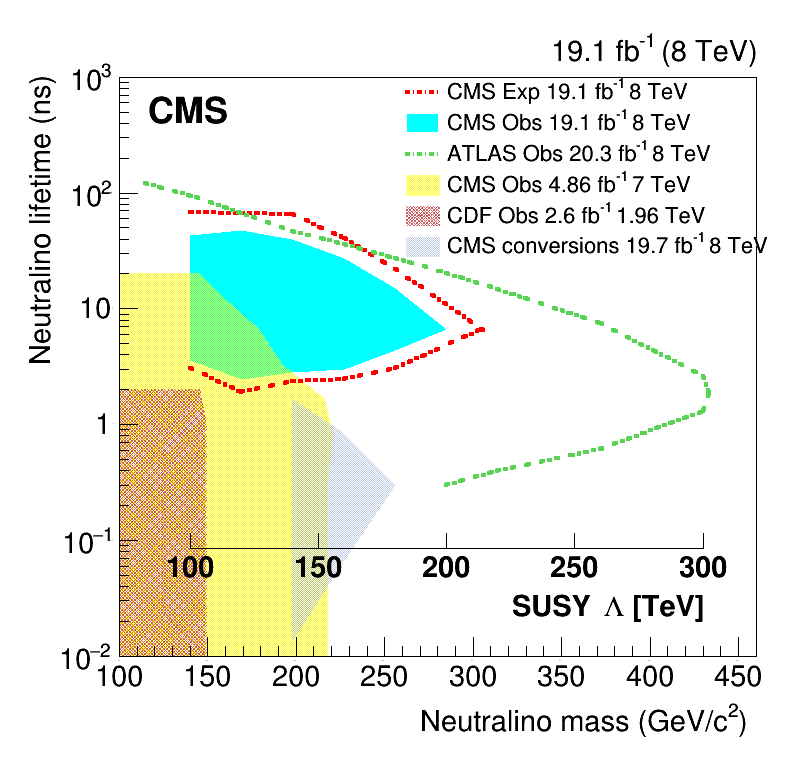
\includegraphics[height=0.85\textwidth, width=0.9\textwidth]{THESISPLOTS/Exclude2D_withAtlas_2015.png}
\captionof{figure}{95\% CL exclusion limit in lightest neutralino mass~(or $\mathbf{\Lambda}$) against mean lifetime in SPS8 benchmark GMSB model. Limits from previous experiments also shown.}
\label{fig:SPS8_2D-Ulimit}
\end{center}
\end{minipage}
\vspace{5mm}

\begin{minipage}{0.95\linewidth}
\begin{center}
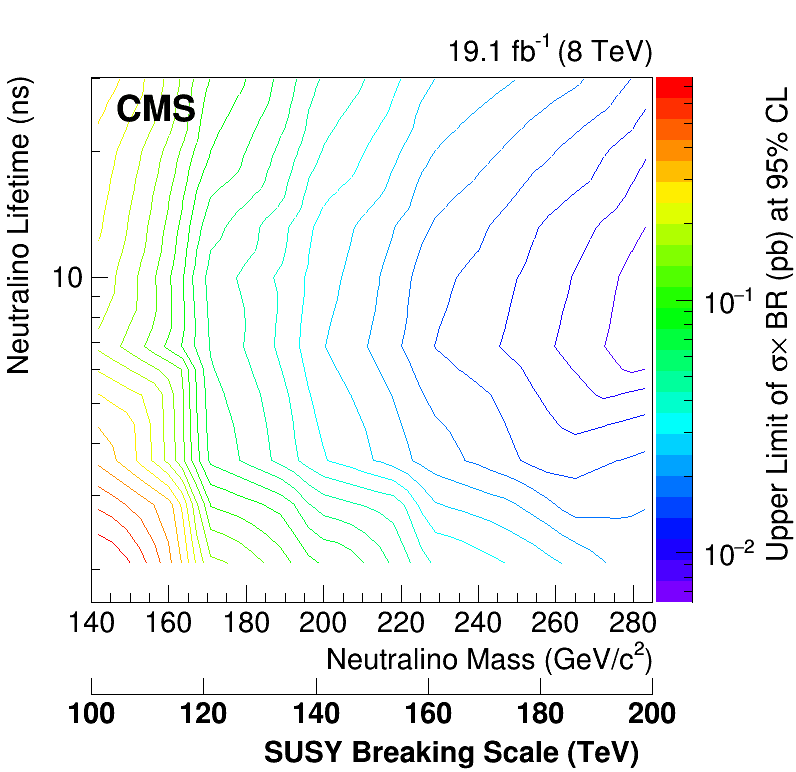
\includegraphics[height=0.85\textwidth, width=0.9\textwidth]{THESISPLOTS/limit2D_Cross-Section-Observed.png}
\captionof{figure}{95\% CL in cross section for different mass and lifetime of the lightest neutralino using the 8\TeV data corresponding to an integrated luminosity of 19.1\fbinv of the CMS experiment.}
\label{fig:SPS8_SIGMA-Ulimit}
\end{center}
\end{minipage}
%%\end{landscape}
%% \clearpage% Flush page
%%}

%%%%%%%%%%%%%%%%%%%%%%%%%%%%%%%%%%%%%%%%%%%%%%%%%%%%%%%%%%%%%%%%%%%%%%%%%%%%%%%%%%%%%%%%%%%%%%%%%%%%%%%
%%%%%%%%%%%%%%%%%%%%%%%%%%%%%%%%%%%%%%%%%%%%%%%%%%%%%%%%%%%%%%%%%%%%%%%%%%%%%%%%%%%%%%%%%%%%%%%%%%%%%%%

\begin{comment}
%%is given in table \ref{tab:SIGNALRES}
%%\vspace{5mm}
%%\begin{minipage}{\linewidth} 
%%\begin{center}
%\begin{table}[ht]
%\renewcommand\arraystretch{1.2}
%%\begin{tabular}{c c}
%%\toprule
%%\hline
%%\bfseries{SPS8 GMSB Signal} & \bfseries {Number of Events}\\
%%\hline
%%\toprule
%%\texttt{GMSB(SPS8)}~($\Lambda=180$~TeV,$c\tau=250$~mm) & $0.2096$ \\
%%\texttt{GMSB(SPS8)}~($\Lambda=180$~TeV,$c\tau=500$~mm) & $4.5423$  \\
%%\texttt{GMSB(SPS8)}~($\Lambda=180$~TeV,$c\tau=1000$~mm) & $6.3646$ \\
%%\texttt{GMSB(SPS8)}~($\Lambda=180$~TeV,$c\tau=2000$~mm) & $6.3968$ \\ 
%%\texttt{GMSB(SPS8)}~($\Lambda=180$~TeV,$c\tau=4000$~mm) & $6.1442$ \\
%%\texttt{GMSB(SPS8)}~($\Lambda=180$~TeV,$c\tau=6000$~mm) & $4.6498$ \\
%%\texttt{GMSB(SPS8)}~($\Lambda=180$~TeV,$c\tau=12000$~mm) & $2.918$ \\
%%\hline 
%%\bottomrule
%%\end{tabular}
%%\captionof{table}{Final number for $\Lambda = 180$\TeV GMSB SPS8 MC signal events  events passing our selection cuts.}
%%\label{tab:SIGNALRES}
%\end{table}
%%\end{center}
%%\end{minipage}
\end{comment}

%%%%%%%%%%%%%%%%%%%%%%%%%%%%%%%%%%%%%%%%%%%%%%%%%%%%%%%
%%%%%%%%%%%%%%%%%%%%%%%%%%%%%%%%%%%%%%%%%%%%%%%%%%%%%%%%%%%%%%%%%%%%%%%%%%%%%%%%
% Possible Future Analysis work!
%%%%%%%%%%%%%%%%%%%%%%%%%%%%%%%%%%%%%%%%%%%%%%%%%%%%%%%%%%%%%%%%%%%%%%%%%%%%%%%%
%\section{Future Improvements}
%%%%%%%%%%%%%%%%%%%%%%%%%%%%%%%%%%%%%%%%%%%%%%%%%%%%%%%%%%%%%%%%%%%%

%%%%%%%%%%%%%%%%%%%%%%%%









%%%%%%%%%%%%%%%%%%%%%%%%%%%%%%%%%%%%%%%%%%%%%%%%%%%%%%%%%%%%%%%%%%%%%%%%%%%%%%%%%%%%%%%%%%%%%%%%%%%%%%%%
\begin{comment}
%%In addition to the $p$-value which is used for quantifying the level of incompatibility between the data and a given hypothesis, the HiggsCombine tool also provides a quantity known as the \textit{significance}~($\mathcal{Z}$). $\mathcal{Z}$ and the $p$-value have a very non-linear relation which can be defined using a two-sided fluctuation if a Gaussian variable $\sigma$, with $5\sigma$ significance corresponding to a $p$-value of $p = 5.7 \times 10^{-7}$ to denote a discovery. Since, we have not observed any significant excess of events over our standard model background, we will not mention a lot about significance in this thesis, but rather talk about $p$-values as they are indispensable in computing limits.
%In summary, our hypothesis test is performed using a given statistical method on each value of a chosen parameter of interest~(POI)(usually denoted $\mu$). The $p$-value is obtained from the sampling distribution of the test statistics being used. Can either obtain this test statistics analytically or through Monte Carlo computation and  numerical integration. By plotting the $p$-value as a function of the POI, we obtain a $p$-value curve~(in this case the $CL_{s} = \frac{CL_{s+b}}{CL_{b}}$).
%The value of $\mu$ which has a p-value $\alpha = 0.05$ is the upper limit~(for 1-dimensional limits, 2-dimensional limits gives lower and upper limits) of $1 - \alpha$  confidence interval~(\ie 95\%).
%\vspace{5mm}
%\begin{minipage}{0.94\textwidth} 
%\begin{center}
%\mbox{
%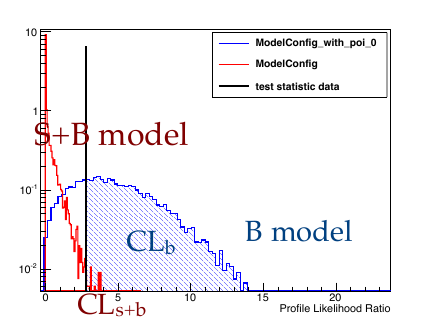
\includegraphics[height=0.65\textwidth, width=0.45\textwidth]{THESISPLOTS/Asymptotics_Test_Stats.png}
%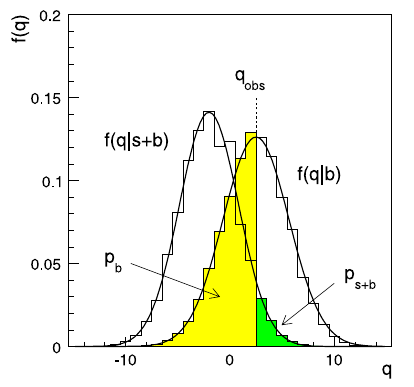
\includegraphics[height=0.615\textwidth, width=0.45\textwidth]{THESISPLOTS/TEST_STATISTICS.png}
%}
%\captionof{figure}{Sampling distributions for $f(t_{\mu}|\mu)$ showing how one extracts the $p$-vlaues. left: is the using a analytic of the Asymptotic method and right: is from the HybridNew method.}
%\label{fig:LIM}
%\end{center}
%\end{minipage}
%\vspace{5mm}
%The important question is always, how does one obtain an expression or a distribution of the test %statistics and $f(t_{\mu}|\mu)$ from the likelihood function? To answer this question, the HiggsCombine tool was developed which consist of various ways of both analytically~(\eg the Asymptotic statistical method \cite{ASYMP}) or through numerical integration or Monte Carlo computation~(\eg the HybridNew statistical method) obtain the test statistics and $ f(t_{\mu}|\mu)$. We have shown the limit computation results of both methods as used in this analysis.
%As an example, the pdf $ f(t_{\mu}|\mu)$ of the test statistics~($t_{\mu}$) obtained though the \textcolor{green}{Asymptotic} statistical method as given in \cite{ASYMP} is:
%\begin{equation}\label{eq:ASYPTOTIC}
%f(t_{\mu}|{\mu}^{\prime}) = \mathbf{\Phi}\left( \frac{\mu -{\mu}^{\prime}}{\sigma}\right)\delta(t_{\mu}) +
 %                            \frac{1}{2}\frac{1}{\sqrt{2\pi}}\frac{1}{t_{\mu}}\exp\left[-\frac{1}{2} %\left(  \sqrt{t_{\mu}} - \frac{\mu - {\mu}^{\prime}}{\sigma}\right)^{2} \right]
%\end{equation}
%where result to a half-chi-square distribution when $\mu = \mu^{\prime}$.

%In subtle point worth mentioning is that in the HybridNew approach, systematics uncertainties are taken into account through the Beyesian prior density $\mathbf{\pi(\theta)}$, and the distribution of the test statistics is computed under the assumption if the Beyesian model of average given as: $$\displaystyle{f(t) = \int f(t|\theta)\pi(\theta)d\theta}$$ and the prior pdf $\mathbf{\pi(\theta)}$ is obtained from some measurements characterized by a given likelihood function $\mathcal{L}_{\mathbf{\theta}}(\mathbf{\theta} )$ which is then used to find the prior using Bayes' Theorem. Unlike other cases where systematic uncertainties are taking as being part of the data and incorporated directly through $\mathcal{G}(\theta)$ as shown in equation \ref{eq:LL}. Nevertheless, they arrive at the same result.
%%%%%%%%%%%%%%%%%%%%%%%%%%%%%%%%%%%%%%%%%%%%%%%%%%%%%%%%%%%%%%%%%%%%%%%%%%%%%% 
%%The accepted method by CMS statistics committee for computing upper upper limit by any search and discovery experiment like ours is to use a profilelikelihood ratio as the test statistics and a mixture of frequentist-hybrid significance test for the test statistics calculator and limit extraction. This method is known as the \textit{HybridNew}  method. The parameters of interests~(POI) in our case are the cross section of signal process and the \textit{nuissance parameters} which are the systematics for the background plus signal model. The sensitivity of the search experiment depends on the systematics and hence the nuissance parameters.
%%%%%%%%%%%%%%%%%%%%%%%%%%
%In a shape based experiment, the mean number of entries in the $i$th bin of the histogram from signal and background will be given as 
%\begin{equation}
%s_{i} = s_{tot} \int_{bin, i} f_{s}\left(t;\mathbf{\theta_{s}}\right) ,\quad 
%b_{i} = b_{tot} \int_{bin, i} f_{b}\left(t;\mathbf{\theta_{b}}\right)
%\end{equation}
%where the functions $f_{s}\left(t;\mathbf{\theta_{s}}\right) $ and $f_{b}\left(t;\mathbf{\theta_{b}}\right) $ are the probability density functions~(Pdfs) of the variable $t$~(ECAL time) for the signal and background events, respectively, and $\mathbf{\theta_{s}} $ and $\mathbf{\theta_{b}} $ represent the parameters which characterize the shapes of the Pdfs. $s_{tot}$ and $b_{tot}$ represents the total mean number of signal and background events, respectively, while each integral gives the probability for an event to be found in bin $i$. $\mathbf{\theta} = \left( \mathbf{\theta_{s}}, \mathbf{\theta_{b}}, b_{tot} \right)$ denote all nuisance parameters~(systematic uncertainties) and $s_{tot}$ is the signal normalization which is fixed to the value predicted by the nominal signal model.

%The $CL_{s}$ method advantage in search experiments where  . The method is used for making statistical inferences by computing the probability or \textit{p-value} from  \textit{test statistics} of the different hypothesis to be tested. From these $p$-values the CL is computed and the exclusion limits derived. The computation of the CL from the results of the hypothesis testing is according to the following procedure:
%%\begin{itemize}
%\item A \textit{Null}~($H_{0}$) and an \textit{Alternate}~($H_{1}$) hypothesis are defined. Additional hypothesis can also be defined, however, in our case we have just two hypothesis to test,
%\item A Test statistics~($t(x)$), where $x$ is the data histogram variable, and its corresponding test %statistics calculator are selected,
%\item The confidence limit is computed by inverting the results of the hypothesis test.
%\end{itemize}
%Before we discuss the limit computation, first, let us describe the CLs technique.
%\par 
%%%%%%%%%%%%%%%%%%%%%%%%%%%%%%%%%%%%%%%%%%%%%%%%%%%%%%%%%%%%%%%%%%%%%
% The acceptance is because it has been tested and validated during the search for the Higgs boson at a previous CERN experiment known as LEP and recently in the discovery of the Higgs boson with mass, $m_{H} = 125.36\pm 0.37(stat.Unc)\pm0.18(syst.Unc)$, in 2012, by both CMS and ATLAS experiments.
%where $s+b$ means signal plus background, $CL_{s+b}$ or $p_{s+b}$ is the $p$-value of the signal plus background hypothesis and $CL_{b}$ or $p_{b}$ is that for the background only hypothesis.
\end{comment}


%%\vspace{5mm}
%%\begin{minipage}{0.94\textwidth} 
%%\begin{center}
%\mbox{
%%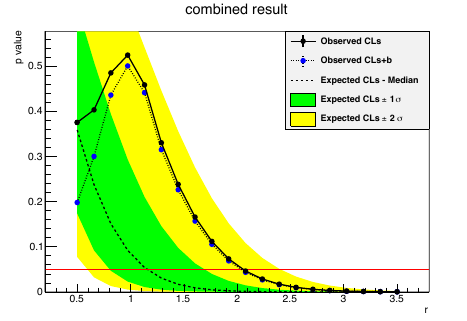
\includegraphics[height=0.45\textwidth, width=0.55\textwidth]{THESISPLOTS/Limits_CLs.png}
%%\captionof{figure}{Distribution of $p$-vlaues showing how upper limit on $\mu$ is extracted for a given threshold probability.}
%%\label{fig:LIMITS_CLS}
%%\end{center}
%%\end{minipage}

